\documentclass[11pt,]{article}
\usepackage[left=1in,top=1in,right=1in,bottom=1in]{geometry}
\newcommand*{\authorfont}{\fontfamily{phv}\selectfont}
\usepackage[]{mathpazo}


  \usepackage[T1]{fontenc}
  \usepackage[utf8]{inputenc}



\usepackage{abstract}
\renewcommand{\abstractname}{}    % clear the title
\renewcommand{\absnamepos}{empty} % originally center

\renewenvironment{abstract}
 {{%
    \setlength{\leftmargin}{0mm}
    \setlength{\rightmargin}{\leftmargin}%
  }%
  \relax}
 {\endlist}

\makeatletter
\def\@maketitle{%
  \newpage
%  \null
%  \vskip 2em%
%  \begin{center}%
  \let \footnote \thanks
    {\fontsize{18}{20}\selectfont\raggedright  \setlength{\parindent}{0pt} \@title \par}%
}
%\fi
\makeatother




\setcounter{secnumdepth}{0}

\usepackage{color}
\usepackage{fancyvrb}
\newcommand{\VerbBar}{|}
\newcommand{\VERB}{\Verb[commandchars=\\\{\}]}
\DefineVerbatimEnvironment{Highlighting}{Verbatim}{commandchars=\\\{\}}
% Add ',fontsize=\small' for more characters per line
\usepackage{framed}
\definecolor{shadecolor}{RGB}{248,248,248}
\newenvironment{Shaded}{\begin{snugshade}}{\end{snugshade}}
\newcommand{\KeywordTok}[1]{\textcolor[rgb]{0.13,0.29,0.53}{\textbf{#1}}}
\newcommand{\DataTypeTok}[1]{\textcolor[rgb]{0.13,0.29,0.53}{#1}}
\newcommand{\DecValTok}[1]{\textcolor[rgb]{0.00,0.00,0.81}{#1}}
\newcommand{\BaseNTok}[1]{\textcolor[rgb]{0.00,0.00,0.81}{#1}}
\newcommand{\FloatTok}[1]{\textcolor[rgb]{0.00,0.00,0.81}{#1}}
\newcommand{\ConstantTok}[1]{\textcolor[rgb]{0.00,0.00,0.00}{#1}}
\newcommand{\CharTok}[1]{\textcolor[rgb]{0.31,0.60,0.02}{#1}}
\newcommand{\SpecialCharTok}[1]{\textcolor[rgb]{0.00,0.00,0.00}{#1}}
\newcommand{\StringTok}[1]{\textcolor[rgb]{0.31,0.60,0.02}{#1}}
\newcommand{\VerbatimStringTok}[1]{\textcolor[rgb]{0.31,0.60,0.02}{#1}}
\newcommand{\SpecialStringTok}[1]{\textcolor[rgb]{0.31,0.60,0.02}{#1}}
\newcommand{\ImportTok}[1]{#1}
\newcommand{\CommentTok}[1]{\textcolor[rgb]{0.56,0.35,0.01}{\textit{#1}}}
\newcommand{\DocumentationTok}[1]{\textcolor[rgb]{0.56,0.35,0.01}{\textbf{\textit{#1}}}}
\newcommand{\AnnotationTok}[1]{\textcolor[rgb]{0.56,0.35,0.01}{\textbf{\textit{#1}}}}
\newcommand{\CommentVarTok}[1]{\textcolor[rgb]{0.56,0.35,0.01}{\textbf{\textit{#1}}}}
\newcommand{\OtherTok}[1]{\textcolor[rgb]{0.56,0.35,0.01}{#1}}
\newcommand{\FunctionTok}[1]{\textcolor[rgb]{0.00,0.00,0.00}{#1}}
\newcommand{\VariableTok}[1]{\textcolor[rgb]{0.00,0.00,0.00}{#1}}
\newcommand{\ControlFlowTok}[1]{\textcolor[rgb]{0.13,0.29,0.53}{\textbf{#1}}}
\newcommand{\OperatorTok}[1]{\textcolor[rgb]{0.81,0.36,0.00}{\textbf{#1}}}
\newcommand{\BuiltInTok}[1]{#1}
\newcommand{\ExtensionTok}[1]{#1}
\newcommand{\PreprocessorTok}[1]{\textcolor[rgb]{0.56,0.35,0.01}{\textit{#1}}}
\newcommand{\AttributeTok}[1]{\textcolor[rgb]{0.77,0.63,0.00}{#1}}
\newcommand{\RegionMarkerTok}[1]{#1}
\newcommand{\InformationTok}[1]{\textcolor[rgb]{0.56,0.35,0.01}{\textbf{\textit{#1}}}}
\newcommand{\WarningTok}[1]{\textcolor[rgb]{0.56,0.35,0.01}{\textbf{\textit{#1}}}}
\newcommand{\AlertTok}[1]{\textcolor[rgb]{0.94,0.16,0.16}{#1}}
\newcommand{\ErrorTok}[1]{\textcolor[rgb]{0.64,0.00,0.00}{\textbf{#1}}}
\newcommand{\NormalTok}[1]{#1}

\usepackage{graphicx,grffile}
\makeatletter
\def\maxwidth{\ifdim\Gin@nat@width>\linewidth\linewidth\else\Gin@nat@width\fi}
\def\maxheight{\ifdim\Gin@nat@height>\textheight\textheight\else\Gin@nat@height\fi}
\makeatother
% Scale images if necessary, so that they will not overflow the page
% margins by default, and it is still possible to overwrite the defaults
% using explicit options in \includegraphics[width, height, ...]{}
\setkeys{Gin}{width=\maxwidth,height=\maxheight,keepaspectratio}

\title{S14 - \emph{Kernel PCA}  }



\author{\Large Juan Carlos Martinez-Ovando\vspace{0.05in} \newline\normalsize\emph{}   \and \Large \vspace{0.05in} \newline\normalsize\emph{ITAM}  }


\date{}

\usepackage{titlesec}

\titleformat*{\section}{\normalsize\bfseries}
\titleformat*{\subsection}{\normalsize\itshape}
\titleformat*{\subsubsection}{\normalsize\itshape}
\titleformat*{\paragraph}{\normalsize\itshape}
\titleformat*{\subparagraph}{\normalsize\itshape}


\usepackage{natbib}
\bibliographystyle{plainnat}
\usepackage[strings]{underscore} % protect underscores in most circumstances



\newtheorem{hypothesis}{Hypothesis}
\usepackage{setspace}

\makeatletter
\@ifpackageloaded{hyperref}{}{%
\ifxetex
  \PassOptionsToPackage{hyphens}{url}\usepackage[setpagesize=false, % page size defined by xetex
              unicode=false, % unicode breaks when used with xetex
              xetex]{hyperref}
\else
  \PassOptionsToPackage{hyphens}{url}\usepackage[unicode=true]{hyperref}
\fi
}

\@ifpackageloaded{color}{
    \PassOptionsToPackage{usenames,dvipsnames}{color}
}{%
    \usepackage[usenames,dvipsnames]{color}
}
\makeatother
\hypersetup{breaklinks=true,
            bookmarks=true,
            pdfauthor={Juan Carlos Martinez-Ovando () and  (ITAM)},
             pdfkeywords = {Kernel methods, singular value decomposition, manifolds.},  
            pdftitle={S14 - \emph{Kernel PCA}},
            colorlinks=true,
            citecolor=blue,
            urlcolor=blue,
            linkcolor=magenta,
            pdfborder={0 0 0}}
\urlstyle{same}  % don't use monospace font for urls

% set default figure placement to htbp
\makeatletter
\def\fps@figure{htbp}
\makeatother



% add tightlist ----------
\providecommand{\tightlist}{%
\setlength{\itemsep}{0pt}\setlength{\parskip}{0pt}}

\begin{document}
	
% \pagenumbering{arabic}% resets `page` counter to 1 
%
% \maketitle

{% \usefont{T1}{pnc}{m}{n}
\setlength{\parindent}{0pt}
\thispagestyle{plain}
{\fontsize{18}{20}\selectfont\raggedright 
\maketitle  % title \par  

}

{
   \vskip 13.5pt\relax \normalsize\fontsize{11}{12} 
\textbf{\authorfont Juan Carlos Martinez-Ovando} \hskip 15pt \emph{\small }   \par \textbf{\authorfont } \hskip 15pt \emph{\small ITAM}   

}

}








\begin{abstract}

    \hbox{\vrule height .2pt width 39.14pc}

    \vskip 8.5pt % \small 

\noindent En la sesion de hoy estudiaremos una variante del analisis de
componentes principales basado en la nocion de similaridad en los datos,
el cual puede ser asociado con estructuras complejas de datos.


\vskip 8.5pt \noindent \emph{Keywords}: Kernel methods, singular value decomposition, manifolds. \par

    \hbox{\vrule height .2pt width 39.14pc}



\end{abstract}


\vskip 6.5pt


\noindent  \section{Intuicion en PCA}\label{intuicion-en-pca}

Recordemos que PCA es un procedimiento de ortogonalizacion de una matriz
de datos \(Y_{(n\times p)}\), con \(n >> p\), basada en la
descomposicion en valores singulares, \[
  Y_{(n\times p)} = 
    U_{(n\times p)} 
    D_{(p\times p)} 
    V_{(p\times p)}.
\]

A partir de esta descomposicion, podemos calcular las siguientes
matrices cuadraticas

\begin{eqnarray}
S_{(p\times p)} & = & Y'_{(n\times p)}Y_{(n\times p)} = V'_{(p\times p)} D^{2}_{(p\times p)} V_{(p\times p)} \\
K_{(n\times n)} & = & Y_{(n\times p)}Y_{(n\times p)}'
= U_{(n\times p)} D^{2}_{(p\times p)} U'_{(p\times n)} 
\end{eqnarray}

La matrix \(S\) corresponde a la sum de cuadrados de \(Y\) --cuando los
datos han sido estandarizados previamente--, mientras que la matriz
\(K\) es referida como la \emph{matriz de Gram}.

Recordemos que el primer componente principalesta dado por la siguiente
transformacion

\begin{eqnarray}
f_1 & = & Y v_{1} \\
    & = & UDV' v_{1} \\
    & = & u_{1} d_{1},
\end{eqnarray}

donde \(v_{1}\) es un vector de dimension \((p\times 1)\)
correspondiente al eigenvector asociado con el primer eigenvalor de
\(Y\).

Como sabemos, el primer componente principal puede obtenerse de tres
formas alternaivas:

\begin{enumerate}
\def\labelenumi{\alph{enumi}.}
\item
  Como el producto de \(Y\) con el primer eigenvector de \(S\)
\item
  A partir de la descomposicion en valores singulaes de \(Y\) (descrito
  lineas arriba)
\item
  A traves de la descomposicion singular de \(K\).
\end{enumerate}

Asi, pues no se necesita saber \(Y\) directamente, sino que basta con
conocer \(S\) o \(K\) para producir los componentes principales de un
conjunto de datos. En particular, el primer componente principal de un
vector \(p\)-dimensional \(y\) puede obtenerse como la proyeccion sobre
eleje del primer componente, i.e. \[
f=v_{1}'y.
\] la expresion anterior puede calcularse directamente, o
\emph{indirectamente} empleando la expresion alternativa \[
f=u_{1}'Yy/d_1=\sum_{i=1}^{n}\left( \frac{u_{i1}}{d_1}\right)y_{i}'y.
\]

Expresiones semjantes se obtienen de manera analoga para los demas
componente principales (no solo el primero).

De esta forma podemos ver que es necesario conocer los productor
interiores \((y_{i}'y)_{i=1}^{n}\) solamente.

Como antes mencionamos, el calculo de \(f_{1}\) puede obtenerse de dos
formas:

\texttt{Forma.1}.- Calcular \(S=Y'Y\), obteniendo el primer eigenvector
de esta matriz, \(v_{i}\) de \(S\), y calcular \[f_{1}=Yv_{1}.\]

\texttt{Forma.2}.- Empleando la matriz de Gram, calculando \(YY'\),
obteniendo el primer eigenvector de esta matriz, \(u_{1}\) y su
correspondiente eigenvalor, \(d_{1}\), y calculando
\[f_{1}=u_{1}d_{1}.\]

La \texttt{Forma.1} es particularmente util cuando \(n>>p\), mientras
que la \texttt{Forma.2} lo es para el caso \(n<<p\).

Al final del dia, PCA descansa en el calculo de los prodcutos interiores
\((y_{i}'y)_{i=1}^{n}\), el cual puede interpretarse como una medida de
`similaridad euclidiana' entre objetos \(p\)-dimensionales.

La idea entonces de \textbf{Kernel PCA} es la de relajar el supuesto de
``similaridad euclidiano'' para otras medidas de similaridad. Esto en
particular cuando los objetos \(y\) residan en \emph{sub-espacios no
lienales} de \(R^{p}\) (curvas, superficies o \emph{manifolds}).

\section{Caracterizacion}\label{caracterizacion}

\textbf{?`Como son esos sub-espacios?}

Veamos un ejemplo con el siguiente diagrama de datos sinteticos.

\begin{Shaded}
\begin{Highlighting}[]
\KeywordTok{set.seed}\NormalTok{(}\DecValTok{1}\NormalTok{)}
\NormalTok{n <-}\StringTok{ }\DecValTok{1000}
\NormalTok{Y <-}\StringTok{ }\KeywordTok{matrix}\NormalTok{(}\KeywordTok{runif}\NormalTok{(n}\OperatorTok{*}\DecValTok{2}\NormalTok{,}\OperatorTok{-}\FloatTok{1.2}\NormalTok{,}\FloatTok{1.2}\NormalTok{),n,}\DecValTok{2}\NormalTok{)}
\NormalTok{r <-}\StringTok{ }\KeywordTok{sqrt}\NormalTok{(}\KeywordTok{apply}\NormalTok{(Y}\OperatorTok{^}\DecValTok{2}\NormalTok{,}\DecValTok{1}\NormalTok{,sum))}
\NormalTok{Y <-}\StringTok{ }\NormalTok{Y[  r}\OperatorTok{<}\NormalTok{.}\DecValTok{25} \OperatorTok{|}\StringTok{ }\NormalTok{(r}\OperatorTok{>}\NormalTok{.}\DecValTok{5} \OperatorTok{&}\StringTok{ }\NormalTok{r}\OperatorTok{<}\NormalTok{.}\DecValTok{75}\NormalTok{) }\OperatorTok{|}\StringTok{ }\NormalTok{r}\OperatorTok{>}\DecValTok{1}\NormalTok{  ,]}
\NormalTok{r <-}\StringTok{ }\KeywordTok{sqrt}\NormalTok{(}\KeywordTok{apply}\NormalTok{(Y}\OperatorTok{^}\DecValTok{2}\NormalTok{,}\DecValTok{1}\NormalTok{,sum))}

\NormalTok{r <-}\StringTok{ }\KeywordTok{sqrt}\NormalTok{(}\KeywordTok{apply}\NormalTok{(Y}\OperatorTok{^}\DecValTok{2}\NormalTok{,}\DecValTok{1}\NormalTok{,sum))}
\NormalTok{clr <-}\StringTok{ }\KeywordTok{rgb}\NormalTok{( (r}\OperatorTok{/}\KeywordTok{max}\NormalTok{(r))}\OperatorTok{^}\NormalTok{.}\DecValTok{7}\NormalTok{,(}\DecValTok{1}\OperatorTok{-}\NormalTok{r}\OperatorTok{/}\KeywordTok{max}\NormalTok{(r))}\OperatorTok{^}\NormalTok{.}\DecValTok{7}\NormalTok{,.}\DecValTok{5}\NormalTok{)}
\KeywordTok{par}\NormalTok{(}\DataTypeTok{mar=}\KeywordTok{c}\NormalTok{(}\DecValTok{3}\NormalTok{,}\DecValTok{3}\NormalTok{,}\DecValTok{1}\NormalTok{,}\DecValTok{1}\NormalTok{),}\DataTypeTok{mgp=}\KeywordTok{c}\NormalTok{(}\FloatTok{1.75}\NormalTok{,.}\DecValTok{75}\NormalTok{,}\DecValTok{0}\NormalTok{))}
\CommentTok{#plot(Y,col=clr)}
\KeywordTok{plot}\NormalTok{(Y)}
\end{Highlighting}
\end{Shaded}

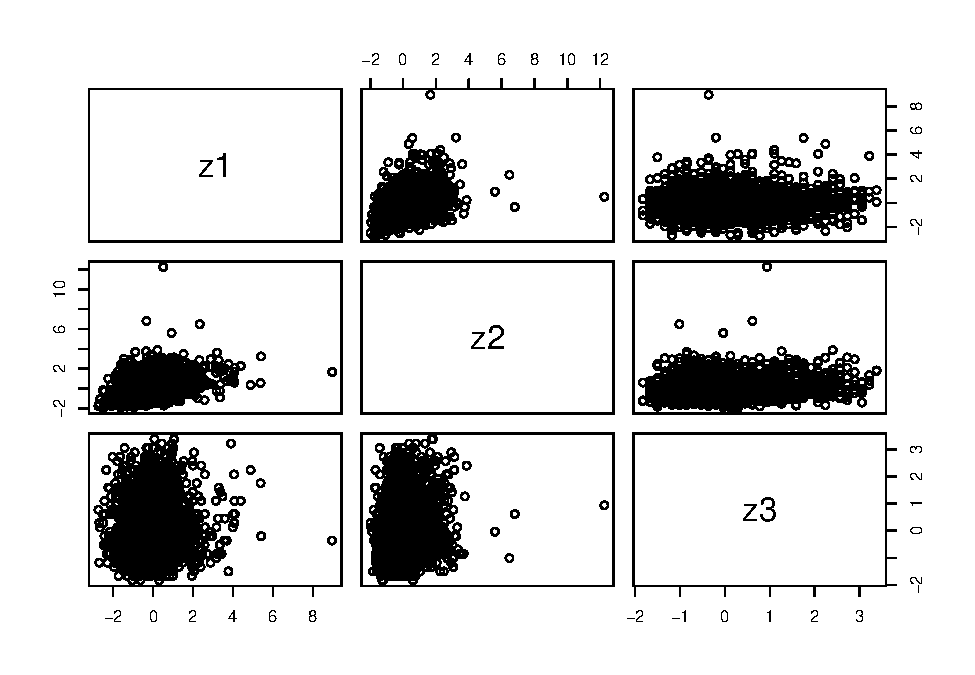
\includegraphics{est46114_s14_kernelpca_files/figure-latex/unnamed-chunk-1-1.pdf}

En este caso, la matriz de Gram deseable sera tal que mida
alternativamente la similaridad entre las \(y_{i}\)s.

\subsection{PCA convencional}\label{pca-convencional}

En caso de realizar PCA convencional en este conjunto de datos, se
obtendrian resultados confusos, pues al parecer no habria
ortogonalizacion que realizar. Veamos los siguientes resultados.

\begin{Shaded}
\begin{Highlighting}[]
\KeywordTok{par}\NormalTok{(}\DataTypeTok{mar=}\KeywordTok{c}\NormalTok{(}\DecValTok{3}\NormalTok{,}\DecValTok{3}\NormalTok{,}\DecValTok{1}\NormalTok{,}\DecValTok{1}\NormalTok{),}\DataTypeTok{mgp=}\KeywordTok{c}\NormalTok{(}\FloatTok{1.75}\NormalTok{,.}\DecValTok{75}\NormalTok{,}\DecValTok{0}\NormalTok{))}
\KeywordTok{plot}\NormalTok{(Y)}
\CommentTok{#plot(Y,col=clr)}
\NormalTok{sY <-}\StringTok{ }\KeywordTok{svd}\NormalTok{(Y)}
\NormalTok{V <-}\StringTok{ }\NormalTok{sY}\OperatorTok{$}\NormalTok{v}
\KeywordTok{abline}\NormalTok{(}\DecValTok{0}\NormalTok{,V[}\DecValTok{2}\NormalTok{,}\DecValTok{1}\NormalTok{]}\OperatorTok{/}\NormalTok{V[}\DecValTok{1}\NormalTok{,}\DecValTok{1}\NormalTok{],}\DataTypeTok{col=}\StringTok{"red"}\NormalTok{)}
\KeywordTok{abline}\NormalTok{(}\DecValTok{0}\NormalTok{,V[}\DecValTok{2}\NormalTok{,}\DecValTok{2}\NormalTok{]}\OperatorTok{/}\NormalTok{V[}\DecValTok{1}\NormalTok{,}\DecValTok{2}\NormalTok{],}\DataTypeTok{col=}\StringTok{"blue"}\NormalTok{)}
\end{Highlighting}
\end{Shaded}

\includegraphics{est46114_s14_kernelpca_files/figure-latex/pca_convencional-1.pdf}

En el grafico anterior, las rectas representan los \emph{ejes del PCA}.
Como observamos, los datos de \emph{componentes principales} son iguales
a \(Y\). Esto es porque la \emph{medida de similaridad} empleada es la
euclidiana. El resultado es, en este caso, una rotacion de \(Y\)
solamente.

\begin{Shaded}
\begin{Highlighting}[]
\NormalTok{sY <-}\StringTok{ }\KeywordTok{svd}\NormalTok{(Y)}
\NormalTok{F <-}\StringTok{ }\NormalTok{sY}\OperatorTok{$}\NormalTok{u}\OperatorTok\KeywordTok{diag}\NormalTok{(sY}\OperatorTok{$}\NormalTok{d)}

\KeywordTok{par}\NormalTok{(}\DataTypeTok{mar=}\KeywordTok{c}\NormalTok{(}\DecValTok{3}\NormalTok{,}\DecValTok{3}\NormalTok{,}\DecValTok{1}\NormalTok{,}\DecValTok{1}\NormalTok{),}\DataTypeTok{mgp=}\KeywordTok{c}\NormalTok{(}\FloatTok{1.75}\NormalTok{,.}\DecValTok{75}\NormalTok{,}\DecValTok{0}\NormalTok{))}
\KeywordTok{layout}\NormalTok{(}\KeywordTok{matrix}\NormalTok{(}\KeywordTok{c}\NormalTok{(}\DecValTok{1}\NormalTok{,}\DecValTok{1}\NormalTok{,}\DecValTok{2}\NormalTok{,}\DecValTok{3}\NormalTok{),}\DecValTok{2}\NormalTok{,}\DecValTok{2}\NormalTok{))}
\KeywordTok{plot}\NormalTok{(F[,}\DecValTok{1}\OperatorTok{:}\DecValTok{2}\NormalTok{])}

\KeywordTok{hist}\NormalTok{(F[,}\DecValTok{1}\NormalTok{],}\DataTypeTok{main=}\StringTok{""}\NormalTok{,}\DataTypeTok{col=}\StringTok{"lightblue"}\NormalTok{)}
\KeywordTok{hist}\NormalTok{(F[,}\DecValTok{2}\NormalTok{],}\DataTypeTok{main=}\StringTok{""}\NormalTok{,}\DataTypeTok{col=}\StringTok{"lightblue"}\NormalTok{)}
\end{Highlighting}
\end{Shaded}

\includegraphics{est46114_s14_kernelpca_files/figure-latex/pca_resultados-1.pdf}

\textbf{Nota:} El resultado anterior se obtiene adoptando la matriz
\(K=YY'\) como la matriz de Gram (i.e.~la matriz de similaridad entre
datos \(y_i\)).

\subsection{PCA por kernel}\label{pca-por-kernel}

Ahora, si modificamos la no nocion de similaridad por la siguiente
metrica, \[
d(y_i,y_j)=\left(y_i'y_j+1\right)^{2},
\] la matriz de Gram asociada seria \[
K=\left(YY'+1\right)^{2}.
\]

En este caso, realizando la descomposicion singular de \(K\) resultaria
en el siguiente PCA.

\begin{Shaded}
\begin{Highlighting}[]
\NormalTok{K <-}\StringTok{ }\NormalTok{(}\KeywordTok{tcrossprod}\NormalTok{(Y) }\OperatorTok{+}\StringTok{ }\DecValTok{1}\NormalTok{)}\OperatorTok{^}\DecValTok{2}

\NormalTok{sK <-}\StringTok{ }\KeywordTok{svd}\NormalTok{(K)}
\NormalTok{F <-}\StringTok{ }\NormalTok{sK}\OperatorTok{$}\NormalTok{u}\OperatorTok\KeywordTok{diag}\NormalTok{(sK}\OperatorTok{$}\NormalTok{d)}

\KeywordTok{layout}\NormalTok{(}\KeywordTok{matrix}\NormalTok{(}\KeywordTok{c}\NormalTok{(}\DecValTok{1}\NormalTok{,}\DecValTok{1}\NormalTok{,}\DecValTok{2}\NormalTok{,}\DecValTok{3}\NormalTok{),}\DecValTok{2}\NormalTok{,}\DecValTok{2}\NormalTok{))}
\KeywordTok{plot}\NormalTok{(F[,}\DecValTok{1}\OperatorTok{:}\DecValTok{2}\NormalTok{])}

\KeywordTok{hist}\NormalTok{(F[,}\DecValTok{1}\NormalTok{],}\DataTypeTok{main=}\StringTok{""}\NormalTok{,}\DataTypeTok{col=}\StringTok{"lightblue"}\NormalTok{)}
\KeywordTok{hist}\NormalTok{(F[,}\DecValTok{2}\NormalTok{],}\DataTypeTok{main=}\StringTok{""}\NormalTok{,}\DataTypeTok{col=}\StringTok{"lightblue"}\NormalTok{)}
\end{Highlighting}
\end{Shaded}

\includegraphics{est46114_s14_kernelpca_files/figure-latex/kpca_convencional-1.pdf}

Como es evidente, los datos tranformados (panel izquierdo en la
grafica), responden la evidente separacion de anillos que visualiamos en
los datos originales.

Las proyecciones de los datos en los \emph{nuevos ejes principales} es
tambien distinta, mostrando sesgo en este caso.

La asociacion entre las regiones de los datos originales, \(Y\), y los
datos transformados, \(F\), se muestra en el siguiente grafico.

\begin{Shaded}
\begin{Highlighting}[]
\KeywordTok{par}\NormalTok{(}\DataTypeTok{mfrow=}\KeywordTok{c}\NormalTok{(}\DecValTok{1}\NormalTok{,}\DecValTok{2}\NormalTok{),}\DataTypeTok{mar=}\KeywordTok{c}\NormalTok{(}\DecValTok{3}\NormalTok{,}\DecValTok{3}\NormalTok{,}\DecValTok{1}\NormalTok{,}\DecValTok{1}\NormalTok{),}\DataTypeTok{mgp=}\KeywordTok{c}\NormalTok{(}\FloatTok{1.75}\NormalTok{,.}\DecValTok{75}\NormalTok{,}\DecValTok{0}\NormalTok{))}
\KeywordTok{plot}\NormalTok{(Y,}\DataTypeTok{col=}\NormalTok{clr)}
\KeywordTok{plot}\NormalTok{(F[,}\DecValTok{1}\OperatorTok{:}\DecValTok{2}\NormalTok{],}\DataTypeTok{col=}\NormalTok{clr)}
\end{Highlighting}
\end{Shaded}

\includegraphics{est46114_s14_kernelpca_files/figure-latex/unnamed-chunk-2-1.pdf}

A continuacion describimos el marco general de descomposicion PCA basado
en kernels.

\section{Kernel PCA}\label{kernel-pca}

Al modificar la nocion de similaridad como antes, se introduce la nocion
de \(kernel\). en un contexto general, el \emph{kernel} servira como la
medida de similaridad. Asi, entre dos puntos \(y_i\) y \(y_j\) la
similaridad en kernel se definira como \[
k(y_i,y_j)=\phi(y_i)'\phi(y_j),
\] donde \(\phi\) es una funcion que mapea de \(\mathbb{R}^{p}\) a
\(\mathbb{R}^{q}\) (donde tipicamente \(q>>p\)).

El kernel, asi definido, puede interpretarse como el producto
interioreuclidiano no de los datos originales \(y_i\)s, sino de los
datos modificados por una cierta funcion \(\phi\).

En el ejemplo anterior, la funcion \(\phi\) empleada es \[
\phi(y)=\left(1,\sqrt(2)y_1,\ldots,\sqrt(2)y_p,y_1^{2},\ldots,y_p^{2},\sqrt{2}y_1 y_2, \ldots, \sqrt{2}y_{p-1}y_{p}\right).
\]

\textbf{Ejercicio:} Verifiquen que \(d(y_i,y_j)\) visto antes es igual a
\(\phi(y_i)'\phi(y_j)\) para todo \(y_i,y_j\) en \(\mathbb{R}^{p}\).

\section{Contextos}\label{contextos}

?`En que contextos \emph{Kernel PCA} es util?

\begin{itemize}
\item
  Procesamiento de textos
\item
  Procesamiento de imagenes
\item
  Procesamiento de audio
\end{itemize}

En \texttt{R} se pueden encontrar varias implementaciones confiables en
el paquete `\texttt{kernlab}.

\textbf{Observacion:} Casi todos los procedimientoes vistos en este
curso donde se emplea el producto interior euclidiano pueden modificarse
para definirse en terminos de \emph{kernels}. Regresion es un ejemplo,
derivando en modelos de expansiones de bases de kernels. Eso lo veremos
en la siguiente semana.

\section{Referencias}\label{referencias}

\begin{itemize}
\item
  \textbf{Wang} (2014) \emph{Kernel Principal Component Analysis and its
  Applications in Face Recognition and Shape Models}
\item
  \textbf{Bishop} (2006) \emph{Pattern Recognition and Machine Learning}
\end{itemize}




\newpage
\singlespacing 
\end{document}
